\documentclass[10pt,letterpaper]{article}
\usepackage[T1]{fontenc}
\usepackage{times,microtype,graphicx,booktabs,float}
\usepackage[font=small,labelfont=bf,labelsep=period,skip=4pt]{caption}
\setlength{\textwidth}{6in}
\setlength{\textheight}{9in}
\setlength{\oddsidemargin}{0.25in}
\setlength{\evensidemargin}{0.25in}
\setlength{\topmargin}{-0.35in}
\setlength{\headheight}{0.15in}
\setlength{\headsep}{0.2in}
\setlength{\parindent}{0pt}
\setlength{\parskip}{4pt}
\setlength{\intextsep}{4pt}
\setlength{\textfloatsep}{9pt}
\newcommand{\reporttitle}[2]{\noindent\rule{\linewidth}{4pt}\par
{\LARGE\bfseries #1\par}\vspace{2pt}\noindent\rule{\linewidth}{1pt}\par
#2\par October 16, 2026\par\vspace{4pt}}
\makeatletter
\renewcommand\section{\@startsection{section}{1}{\z@}{9pt}{4pt}{\large\bfseries}}
\makeatother
\renewenvironment{abstract}{\small\textbf{Abstract}\par}{\par\vspace{3pt}}
\let\originalitemize\itemize
\renewcommand{\itemize}{\originalitemize\setlength{\itemsep}{1pt}\setlength{\parskip}{0pt}\setlength{\parsep}{0pt}}
\let\originalenumerate\enumerate
\renewcommand{\enumerate}{\originalenumerate\setlength{\itemsep}{1pt}\setlength{\parskip}{0pt}\setlength{\parsep}{0pt}}
\begin{document}
\reporttitle{Alignment package comparison}{Arabidopsis SE/PE DAP and bulk ATAC; BWA-MEM2, BWA and Bowtie2}
\begin{abstract}At the 1-million-pair cap, Bowtie2 gives peak-base Jaccard values of 0.5611 to 0.8493 against BWA-MEM2 across four PE DAP treatments. At the deeper SE DAP cap, FUS3 motif support is 466/998 baseline windows versus 465/998 Bowtie2 windows. These measurements describe agreement and independent motif support, not a validated accuracy ranking. We would retain BWA-MEM2 pending broader evidence.\end{abstract}
\section*{Setup}
\textbf{Comparisons.} BWA-MEM2 2.3, BWA 0.7.19 and Bowtie2 2.5.5 use the same sampled reads and declared reference. The BWA-MEM2 package reports an older banner; recorded binary identity establishes the package version. Bowtie2 uses very-sensitive-local and a 2,000-base maximum PE insert; ATAC also allows dovetail and disables mixed/discordant pairs.

\textbf{Scoring.} Peak Jaccard is base-pair intersection/union against baseline peaks. Fixed-region Spearman compares fragment counts on identical baseline regions. PBM support counts motif-positive 200-base summit windows with same-chromosome, GC-matched controls. These operating policies are not a pure binary substitution.

\begin{table}[H]\centering\small\caption{Input identities at the dap-pe-1m cap.}
\begin{tabular}{lrr}\toprule
Library & Role / control & Raw templates \\ \midrule
SRR31238993 & Control & 1,000,000 \\
SRR31238589 & SRR31238993 & 1,000,000 \\
SRR31239194 & SRR31238993 & 1,000,000 \\
SRR31238722 & SRR31238993 & 1,000,000 \\
SRR31238919 & SRR31238993 & 1,000,000 \\
\bottomrule\end{tabular}\end{table}
\section{Bowtie2 changes peak agreement unevenly across treatments}
Across 4 PE treatments, fixed-region Spearman spans 0.8793 to 0.9269 for Bowtie2. The 2 lower-peak-count libraries have Jaccard below 0.58, compared with more than 0.82 for the other 2 treatments.

\begin{figure}[H]\centering\makebox[\linewidth][c]{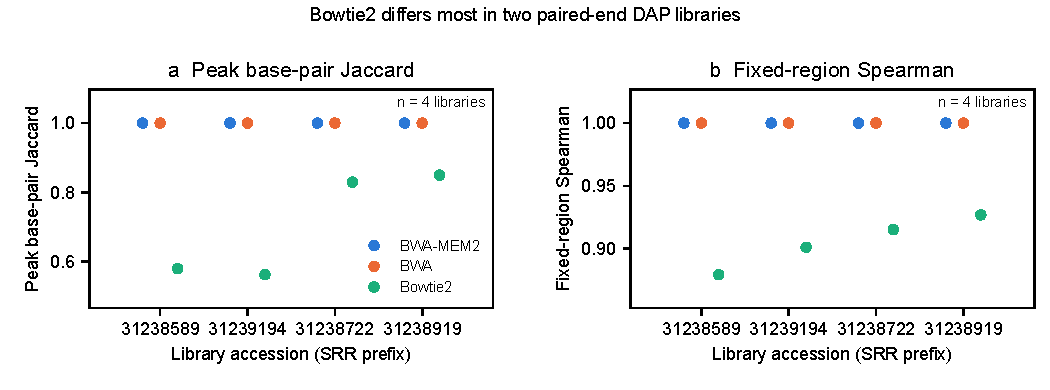
\includegraphics[width=7in]{figures/alignment-quality.pdf}}
\caption{Peak and fixed-region agreement at the 1-million-pair cap.}\end{figure}
\newpage
\section{Independent motif support does not favor a general aligner change}
The deeper SE DAP comparison covers 2 transcription factors, not 1,998 independent experiments. FUS3 has 2 unmatched control windows, so its top-ranked denominator is 998 rather than 1,000.

\begin{table}[H]\centering\small\caption{Independent PBM support in matched top-ranked windows.}
\begin{tabular}{lrrr}\toprule
Library & Method & Motif hits / windows & Control hits \\ \midrule
SRR2926076 & bwa & 466/998 & 12 \\
SRR2926076 & bowtie2 & 465/998 & 13 \\
SRR2926076 & baseline & 466/998 & 12 \\
SRR2926841 & bwa & 581/1000 & 16 \\
SRR2926841 & bowtie2 & 581/1000 & 16 \\
SRR2926841 & baseline & 581/1000 & 16 \\
\bottomrule\end{tabular}\end{table}
\begin{figure}[H]\centering\makebox[\linewidth][c]{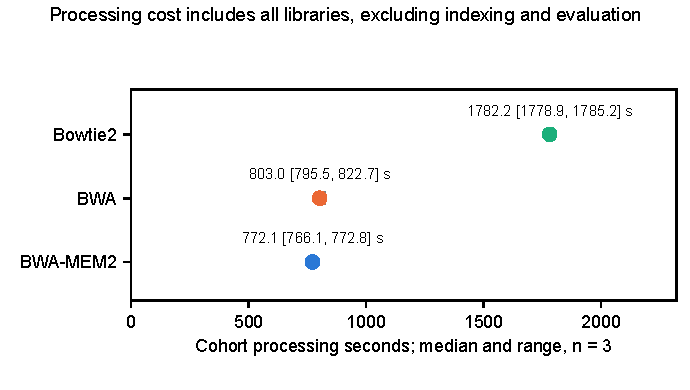
\includegraphics[width=4.6in]{figures/alignment-cost.pdf}}
\caption{Fresh PE DAP cohort timings at the 1-million-pair cap.}\end{figure}
\section*{Open issues}
\begin{itemize}
\item One species and selected TFs cannot establish a universal aligner ranking.
\item Bowtie2 local alignment and pairing policies differ from BWA policies.
\item Timings cover all cohort libraries, exclude indexing and evaluation, and allow 14 tool CPUs.
\end{itemize}
\section*{Recommendation}
We would retain BWA-MEM2 and investigate disagreement on held-out biological evidence.

\begin{enumerate}
\item Expand TF and read-length coverage.
\item Inspect alternative-specific peaks before accepting greater retention as improvement.
\end{enumerate}
\section*{Appendix: Methods}
We summarize recorded results without rerunning biological processing. The main Arabidopsis matrix uses seeded nested raw-template subsets (seed 60141), three fresh technical repetitions at the 1-million cap and one at the 5-million cap. Actual counts replace requested caps for short libraries. DAP retains primary mapped reads including MAPQ 0; ATAC selects proper primary pairs with both mates MAPQ at least 30, excludes MAPQ 255, organelles and marked duplicates. Biological identity is preserved. Source files are SHA-256 checked against the accompanying catalog; evidence snapshot revision ed1c50b8e4b5 includes the October 13 to 16 records. Completed local reference assessments are separately identified in that catalog.

\end{document}
